\section{Theoretische Grundlagen}
Ziel dieses versuches ist es mithilfe des Faraday-Effektes die effektive Masse der Leitungselektronen in 
Galium-Arsenit zu bestimmen. \\
\\
Der Faraday-Effekt, der auch als Faraday-Rotation bezeichnet wird, beschreibt die Drehung der
Polarisationsrichtung einer linear polarisierten Welle bei dem Durchgang durch ein Medium 
unter dem Einfluss eines äußeren Magnetfeldes. Mithilfe dieses Effektes ist es möglich die 
Bandstruktur unterschiedlicher Materialien zu verstehen. \\

\subsection{Beschreibung der Bandstruktur}
Wenn über die Bandstruktur gesprochen wird, ist die Rede von einem Valenz- und einem Leiterband. 
Dabei entspricht das Valenzband dem höchsten besetzten Energieband. Das Energieband, das sich über dem 
Valenzband befindet, wird als Leiterband bezeichnet. \\
Diese Energiebänder entstehen aufgrund hinreichend großer Annäherung von Atomen. Dadurch kommt es zum 
Überlappen der Atomorbitale und durch die Superposition dieser zur Entstehung der Energiebänder. \\
Anhand der Energiebänder ist es möglich Materialien in Isolatoren, Halbleiter und Metalle zu unterteilen. 
In Abbildung \ref{fig:Bandstrukturen} sind die unterschiedlichen Bandstrukturen schematisch abgebildet.
\begin{figure}[H]
    \centering
    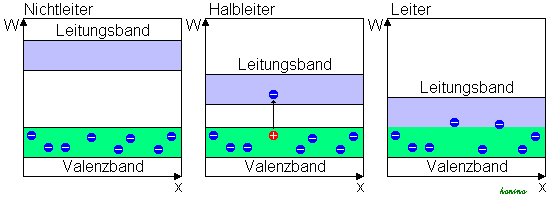
\includegraphics[width=0.8\textwidth]{images/Bandstruktur.png}
    \caption{Schematische Darstellung der unterschiedlichen Bandstrukturen. Links ist die Bandstruktur eines Isolators, 
    in der Mitte die eines Halbleiter und rechts eines Metalls abgebildet \cite{BS}.}
    \label{fig:Bandstrukturen}
\end{figure} \noindent
Es wird deutlich, dass bei einem Isolator, der auf der rechten Seite abgebildet ist, ein Abstand zwischen 
dem Leitungs- und dem Valenzband vorliegt. Diese wird als Bandlücke bezeichnet. Bei einem Isolator ist diese
Bandlücke zu groß, um sie allein mithilfe von thermischer Energie überwinden zu können. Das hat zur Folge, 
dass keine Elektronen in das Leitungsband gehoben werden und somit eine elektrische Leitfähigkeit erzeugen könnten. 
Bei einem Halbleiter, wie es auch Galium-Arsenit ist, liegt ebenfalls eine Bandlücke vor. Diese ist im Vergleich 
zu der eines Isolators kleiner. Somit können hier mithilfe von thermischer Energie Elektronen in das Leitungsband 
gehoben werden und das entsprechende Material wird leitend. Mithilfe von Dotierungen können die Bandlücken 
von Halbleitern verkleinert werden. Dazu werden Ladungsträger in das Material eingefügt. Dabei wird zwischen 
n- und p-Dotierung unterschieden. Bei einer n-Dotierung werden Elektronen-Donatoren, wohingegen bei einer p-Dotierung
Elektronen-Akzeptoren in das Material eingefügt werden. Diese sorgen dann für eine veränderte Bandstruktur, diese 
ist in Abbildung \ref{fig:BS_neu} dargestellt. \\
\begin{figure}[H]
    \centering
    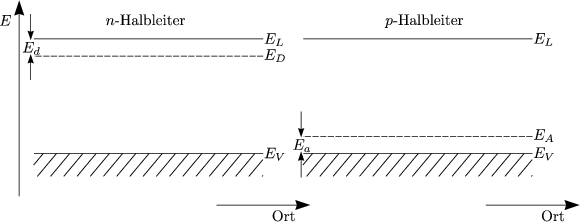
\includegraphics[width=0.8\textwidth]{images/BS_neu.png}
    \caption{Abbildung der durch eine Dotierung veränderten Bandstruktur eines Halbleiters. Links ist die n-Dotierung und rechts 
    die p-Dotierung dargestellt \cite{BS_neu}.}
    \label{}
\end{figure} \noindent
Bei einem Metall liegt kein Bandlücke vor. Außerdem ist das Leitungsband bereits zum Teil gefüllt. Somit reichen
bereits beliebig kleine Feldstärken aus, damit Elektronen in einen höheren Zustand übergehen können. Sie können 
als frei angenommen werden. 